% Vektorgrafiken der Lesefassung. Die Edition lädt TikZ.
\definecolor{differencesblue}{RGB}{34,92,133}
\definecolor{differencesgreen}{RGB}{49,112,81}
\definecolor{differencesgray}{RGB}{104,111,119}

\newcommand{\DifferencesPairGrid}{%
  \par\medskip\noindent
  \begin{minipage}{\linewidth}
  \centering
  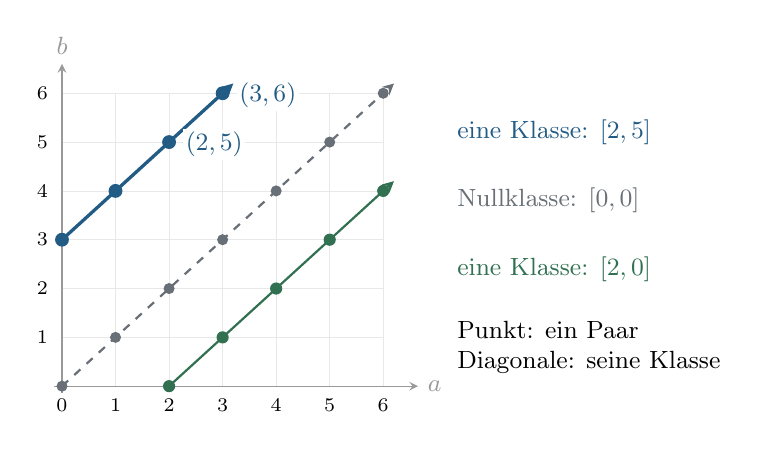
\begin{tikzpicture}[x=.68cm,y=.62cm,font=\small,>=stealth]
    \draw[step=1,gray!18,very thin] (0,0) grid (6,6);
    \draw[->,gray!80] (-.15,0)--(6.65,0) node[right] {\(a\)};
    \draw[->,gray!80] (0,-.15)--(0,6.6) node[above] {\(b\)};
    \foreach \k in {0,...,6} {
      \node[below,font=\scriptsize] at (\k,-.07) {\(\k\)};
    }
    \foreach \k in {1,...,6} {
      \node[left,font=\scriptsize] at (-.08,\k) {\(\k\)};
    }

    \draw[->,differencesgray,dashed,thick] (0,0)--(6.2,6.2);
    \draw[->,differencesgreen,thick] (2,0)--(6.2,4.2);
    \draw[->,differencesblue,very thick] (0,3)--(3.2,6.2);
    \foreach \k in {0,...,6} {
      \fill[differencesgray] (\k,\k) circle (2pt);
    }
    \foreach \a/\b in {2/0,3/1,4/2,5/3,6/4} {
      \fill[differencesgreen] (\a,\b) circle (2.2pt);
    }
    \foreach \a/\b in {0/3,1/4,2/5,3/6} {
      \fill[differencesblue] (\a,\b) circle (2.5pt);
    }
    \node[anchor=west,text=differencesblue,fill=white,inner sep=1pt]
      at (2.25,4.95) {\((2,5)\)};
    \node[anchor=west,text=differencesblue,fill=white,inner sep=1pt]
      at (3.25,5.95) {\((3,6)\)};

    \node[anchor=west,text=differencesblue] at (7.2,5.2)
      {eine Klasse: \([2,5]\)};
    \node[anchor=west,text=differencesgray] at (7.2,3.8)
      {Nullklasse: \([0,0]\)};
    \node[anchor=west,text=differencesgreen] at (7.2,2.4)
      {eine Klasse: \([2,0]\)};
    \node[anchor=west,align=left] at (7.2,.8)
      {Punkt: ein Paar\\Diagonale: seine Klasse};
  \end{tikzpicture}
  \par\smallskip\small\raggedright
  Ein Ausschnitt aus \(\mathbb N\times\mathbb N\).
  Die Gitterpunkte auf derselben Diagonalen erfüllen die
  Kreuzsummengleichung. Hervorgehoben sind drei Klassen; jede setzt
  sich außerhalb des gezeichneten Ausschnitts fort. Die blauen Paare
  \((2,5)\) und \((3,6)\) sind verschiedene Elemente derselben Klasse.
  \end{minipage}\par\medskip
}

\newcommand{\DifferencesEmbeddingDiagram}{%
  \par\medskip\noindent
  \begin{minipage}{\linewidth}
  \centering
  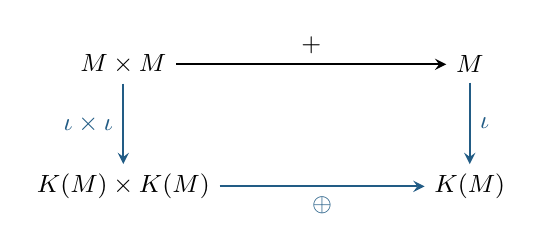
\begin{tikzpicture}[x=1cm,y=1cm,font=\small,>=stealth]
    \node (natpair) at (0,1.55) {\(M\times M\)};
    \node (nat) at (4.4,1.55) {\(M\)};
    \node (intpair) at (0,0) {\(K(M)\times K(M)\)};
    \node (int) at (4.4,0) {\(K(M)\)};
    \draw[->,thick] (natpair)--node[above] {\(+\)}(nat);
    \draw[->,thick,differencesblue]
      (intpair)--node[below] {\(\oplus\)}(int);
    \draw[->,thick,differencesblue]
      (natpair)--node[left] {\(\iota\times\iota\)}(intpair);
    \draw[->,thick,differencesblue]
      (nat)--node[right] {\(\iota\)}(int);
  \end{tikzpicture}
  \par\smallskip\small\raggedright
  Beide Wege führen zum selben Ergebnis: Man kann zuerst \(a\) und
  \(b\) in \(M\) verknüpfen und dann einbetten oder zuerst
  beide Elemente einbetten und ihre Klassen verknüpfen.
  Dabei bedeutet \((\iota\times\iota)(a,b)=(\iota(a),\iota(b))\).
  \end{minipage}\par\medskip
}
